\documentclass{report}
\usepackage[utf8]{inputenc}
\usepackage{xcolor}

\usepackage{filecontents}
\usepackage{tabularx}
\usepackage{csquotes}
\usepackage{hyperref}
\usepackage{parskip}
\usepackage{graphicx}
\usepackage{subcaption}

% Now also shows subsub section ect. in the table of contents
\setcounter{secnumdepth}{3}

% Create \fullref command
\newcommand*{\fullref}[1]{\hyperref[{#1}]{\textcolor{blue}{\underline{\ref*{#1} \nameref*{#1}}}}}

\begin{filecontents}{\jobname.bib}
@techreport{techreport,
  author = {John Dough and Jane Doe},
  title = {An example of some basic analysis},
  submissiondate = {2013/01/22},
  year = {2013},
  urldate = {2014-04-10},
  url = {http://example.com/2013/example_semester_report_12.pdf}
}
\end{filecontents}

\usepackage[style=numeric, backend=biber]{biblatex}
\addbibresource{\jobname.bib}

\title{Modular monolith}

\author{Jessie Liauw A Fong}

\begin{document}

\maketitle
\tableofcontents

\chapter{Preface}
I am Jessie Liauw A Fong, 20 years old. I was born in Amsterdam but moved to Zaandam and still live there. I started programming in 2010 when I was in the first class of middle school. After a year of programming my interest stagnated but in 2015 I chose to begin the study software engineering and I immediately felt that passion again and I haven’t lost that pasion since. In the end of 2015 I started my first software engineering job at The EsportsWall. This was a voluntary job because I did not have enough skills to get paid. 3 months later I did to start my internship at Endouble. I worked at Endouble for 1 year. 5 months as an intern and 7 months as an part time employee.

After I finished my internship at Endouble I started by own company JCB Development. Where I build high-end websites.

At the end of my time at Endouble I started a new parttime internship at Ximedes where I learned a lot about infrastructure. This is also the company I met my now co-worker Erik Schouten. He worked at CargoLedger and that is also where I work now. In the beginning of September 2018 I started a new company together with Stijn Claessen and Siebe Goos called EFFE Planning. This is also the company I will do my thesis in.

This thus means I know the ins and outs of the company.

\chapter{Summary}

\chapter{Introduction}

\section{Motive}
EFFE as a company uses the SaaS model in order to comply to it’s expected growth. The basic SaaS model includes the basic application or MVP. This is in order to keep the application as abstract as possible. So that every company can connect their scheduling procedure to EFFE. But EFFE also wants to cater to the needs of bigger clients. This is why we created building blocks.

Building blocks are features that can be added/removed from the application. This can be done by the user or by EFFE. Examples of building blocks are white labeling, integration with frontend system and payroll integration. These building blocks are not required when acquiring EFFE but can be added one by one.

\section{Intention}
So the question is how are we going to implement these building blocks. We have a few requirements:
\begin{itemize}
	\item They need to be interchangeable. Meaning the same building block can be changed with another one that does the same job with maybe extra functionality.
	
	\item They should be able to do everything programming related. From if else to database calls.
	
	\item They have impact on the frontend as well as the backend
	
	\item Building block should be completely separate from the application (loosely coupled)
\end{itemize}

\chapter{Research design}
This chapter contains the information on how the research will be conducted.

\section{Research objective}

\subsection{The problem}
Right now EFFE is developing an application for employment agencies in which those employment agencies can schedule their employees automatically. The current application is really basic and there are requests from potential clients to implement certain features. We decided to add something to the business model called building blocks.

\begin{displayquote}
	\large{"Building blocks are interchangeable implementations of business logic that can be reused as efficient as possible"}
\end{displayquote}

EFFE is looking how to implement the building blocks in such a manner where scalability and maintainability are the focus.

\subsection{Objective}
The objective is to create a recommendation for an infrastructure on how to create and maintain that infrastructure. Where the focus lays on interchangeability and scalability of the different functionalities.

\begin{tabularx}{\linewidth}{|>{\hsize=.3\hsize}X|
		>{\hsize=.7\hsize}X|}
	\hline
	Stakeholder &
	Interest to the objective
	\\
	\hline
	EFFE &
	The obvious stakeholder is EFFE. EFFE will enhance its business model. But not only that. We will also create a better infrastructure which means that we can implement functionalities faster and cater more to the clients’ need.
	\\
	\hline
	Client &
	The client is also the one interested in this process. They are probably not interested into what happens behind the scenes but they are interested in the possibilities it adds for them to EFFE’s application
	\\
	\hline
\end{tabularx}

\section{Research framework}

\subsection{Objects}
This chapter describes who/what the objects are for this research and why.

\subsubsection{Backend architecture}
Arguably the most important object is the backend architecture. There is already a lot of research available regarding backend architecture. The backend is also the place where the business logic will be expressed. The backend connects to the database and thus needs a lot of attention when creating this section of the application.

\subsubsection{Frontend architecture}
The second object, frontend architecture, is a lesser known subject when looking at modularity of the actual system. Most of the big companies have a single frontend application per platform.

\subsubsection{Deployment lane}
The backend and the frontend are the software side of the equation but the hardware is also important. Where does the software run? How does it run? The deployment lane is the section that pieces it all together. This object creates the hardware or virtual hardware. Sets this hardware up so it can then proceed to deploy the frontend and backend on the just created hardware. This process is very important and EFFE is not the first company wanting to adopt this. Which means there is already a lot of research in this area.

\subsubsection{Project manager}
\label{sec:ProjectManager}
The last object we want to research is the project manager. Because the research is focussed on implementing business logic in a modular way it is important to research what can go wrong when the business logic is translated to code.

\subsection{Research perspective}
The research perspective is straight forward. Because I am one of the founders of EFFE and I am also doing this research in name of EFFE it has my best interest to approach this research from the side of EFFE. This means that I will put more emphasis on sustainability than for example on the performance. Because for now performance can be dealt with later but if you want something to be sustainable you have to think about it from the ground up. Otherwise you will need to rewrite the whole architecture.

\subsection{Research sources}
This section will describe which sources will be used when evaluating the research objects. This will not include everything but a broad spectrum of the sources that may be used in the research:

\begin{itemize}
	\item \textbf{Modular architecture books: }In the end everything I need to know all comes down to modular programming. Modular programming is a very broad term and it is important to find how someone else may look at this term.
	
	\item \textbf{Implementations of modular programming: }Theory is one side of the coin. Everything can work perfectly in theory but when implementing the theoretic side you will find problems you haven't thought of before.
	
	\item \textbf{Critique from outside: }It is known that software architecture is an opinion based subject. This is because especially this area of software is fairly young. Software architecture did not have a lot of time to develop itself as far as some other aspects of software engineering such as operating systems. Because software architecture is young there are a lot of people voicing their opinions and it is important to look at the criticism on some of the architectures.
	
	\item \textbf{Researches on deployment of architecture: }I will be researching more than one architecture. Each architecture has its own development environment and deployment environment. The architecture of the servers on which the program runs is important but that will be heavily influenced by the architecture of the software. Nevertheless should it be researched separately from the software architecture
\end{itemize}

\subsection{Evaluation criteria}
These are the criteria or leading questions that will be asked to research objects. Note: not all evaluation criteria apply to all research objects:

\begin{itemize}
	\item \textbf{What is the biggest pitfall when implementing business logic: }As mentioned in \fullref{sec:ProjectManager} there will also be considered how business logic is translated to code. Because the building blocks will eventually be different based on business logic. The research will include what can go wrong in which way.
	
	\item \textbf{What are the most used architectures in this area: }There is always a reason why one architecture is very common and the other one isn't. In the research the reasoning will be extracted and reflected on.
	
	\item \textbf{What are the most upcoming architectures that are focused on modularity: }Again the whole research is based on the building blocks. These modular functionalities that can be designed via a common interface. Which architecture has which solution for this?
	
	\item \textbf{Which programming languages has the best attributes to complement the modularity: }Some languages are written purely for scripting or some are written to be focused on implementing algorithms more easily. Each programming language has its attributes and which of these attributes are most defining and important to a modular system.
	
	\item \textbf{Which quality attributes are deemed most important to EFFE?: }The quality attributes from ISO 205010 \cite{techreport} are the backbone of an the architecture. In the research will describe which are most important to EFFE. It is then important to reflect the quality attributes we chose on the architectures.
\end{itemize}

\subsubsection{Research framework}

\begin{figure}[h!]
	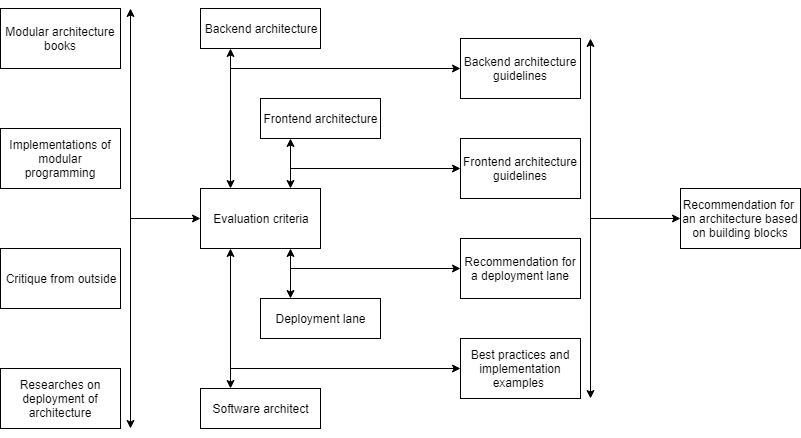
\includegraphics[width=\linewidth]{research_framework.png}
	\caption{Research framework}
\end{figure}

\chapter{Sources}

\printbibliography[heading=none]

\end{document}